\documentclass{beamer}
\usepackage[utf8]{inputenc}
\usepackage[T1]{fontenc}
% \usepackage{amscd, amsfonts, amsmath, amssymb, amstext, amsthm, caption, epsfig, fancyhdr, float, graphicx, latexsym, mathtools, multicol, multirow, algorithm, chngcntr}
\usepackage[english, french]{babel}
\usepackage{booktabs}

\usepackage{amsmath,amssymb}
\usepackage{graphicx}
\usepackage{caption}
\usepackage{subfig}
\usepackage{xspace}
\usepackage{fourier}

\usepackage{tikz}
\usetikzlibrary{shapes,arrows}
\usepackage{tkz-graph}
\usetikzlibrary{automata,arrows,positioning,calc}
\usetikzlibrary{positioning}
\usetikzlibrary{fit}
\usetikzlibrary{backgrounds}
\usetikzlibrary{calc}
\usetikzlibrary{shapes}
\usetikzlibrary{mindmap}
\usetikzlibrary{decorations.text}
\usetikzlibrary{snakes}

% \theoremstyle{definition} % insert bellow all blocks you want in normal text
% \newtheorem{definition}{Definition}



% tikzmark command, for shading over items
\newcommand{\tikzmark}[1]{\tikz[overlay,remember picture] \node (#1) {};}
% Define block styles
\tikzstyle{decision} = [diamond, draw, fill=blue!20,
    text width=4.5em, text badly centered, node distance=3cm, inner sep=0pt]
\tikzstyle{block} = [rectangle, draw, fill=blue!20,
    text width=5em, text centered, rounded corners]
\tikzstyle{line} = [draw]
\tikzstyle{cloud} = [draw, ellipse,fill=red!20, node distance=3cm,
    minimum height=2em]

\usepackage[most]{tcolorbox}

\setbeamertemplate{blocks}[rounded][shadow=true] % use rounded blocks with standard beamer shadow


% Distributions.
\newcommand*{\UnifDist}{\mathsf{Unif}}
\newcommand*{\ExpDist}{\mathsf{Exp}}
\newcommand*{\DepExpDist}{\mathsf{DepExp}}
\newcommand*{\GammaDist}{\mathsf{Gamma}}
\newcommand*{\LognormalDist}{\mathsf{LogNorm}}
\newcommand*{\WeibullDist}{\mathsf{Weib}}
\newcommand*{\ParetoDist}{\mathsf{Par}}
\newcommand*{\NormalDist}{\mathsf{Norm}}

\newcommand*{\GeometricDist}{\mathsf{Geom}}
\newcommand*{\NegBinomialDist}{\mathsf{NegBin}}
\newcommand*{\PoissonDist}{\mathsf{Poisson}}
\newcommand*{\BivariatePoissonDist}{\mathsf{BPoisson}}
\newcommand*{\CyclicalPoissonDist}{\mathsf{CPoisson}}

\newcommand*{\iid}{\textbf{iid}\@\xspace}
\newcommand*{\pdf}{\textbf{pdf}\@\xspace}
\newcommand*{\cdf}{\textbf{cdf}\@\xspace}
\newcommand*{\pmf}{\textbf{pmf}\@\xspace}
\newcommand*{\abc}{{\textbf{abc}}\@\xspace}
\newcommand*{\smc}{\textbf{smc}\@\xspace}
\newcommand*{\mcmc}{\textbf{mcmc}\@\xspace}
\newcommand*{\ess}{\textbf{ess}\@\xspace}
\newcommand*{\mle}{\textbf{mle}\@\xspace}
\newcommand*{\bic}{\textbf{bic}\@\xspace}
\newcommand*{\kde}{\textbf{kde}\@\xspace}
\newcommand*{\glm}{\textbf{glm}\@\xspace}
\newcommand*{\xol}{\textbf{xol}\@\xspace}
\newcommand*{\cpu}{\textbf{cpu}\@\xspace}
\newcommand*{\gpu}{\textbf{gpu}\@\xspace}
\newcommand*{\arm}{\textbf{arm}\@\xspace}

\def \si {\sigma}
\def \la {\lambda}
\def \al {\alpha}
% \def\e*{\end{eqnarray*}}
\def \di{\displaystyle}

\def \E{\mathbb E}
\def \N{\mathbb N}
\def \Z{\mathbb Z}
\def \NZ{\mathbb{N}_0}
\def \I{\mathbb I}
\def \w{\widehat}
\def \P {\mathbb P}
\def \V{\mathbb V}


\newcommand{\CL}{\mathbb{C}}
\newcommand{\RL}{\mathbb{R}}
\newcommand{\nat}{{\mathbb N}}
\newcommand{\Laplace}{\mathscr{L}}
\newcommand{\e}{\mathrm{e}}
\newcommand{\ve}{\bm{\mathrm{e}}} % vector e

\renewcommand{\L}{\mathcal{L}} % e.g. L^2 loss.

\newcommand{\ih}{\mathrm{i}}
\newcommand{\oh}{{\mathrm{o}}}
\newcommand{\Oh}{{\mathcal{O}}}
\newcommand{\Exp}{\mathbb{E}}

\newcommand{\Norm}{\mathcal{N}}
\newcommand{\LN}{\mathcal{LN}}
\newcommand{\SLN}{\mathcal{SLN}}

\renewcommand{\Pr}{\mathbb{P}}
\newcommand{\Ind}{\mathbb I}
\newcommand\bfsigma{\bm{\sigma}}
\newcommand\bfSigma{\bm{\Sigma}}
\newcommand\bfLambda{\bm{\Lambda}}
\newcommand{\stimes}{{\times}}
\def \limsup{\underset{n\rightarrow+\infty}{\overline{\lim}}}
\def \liminf{\underset{n\rightarrow+\infty}{\underline{\lim}}}




% vertical separator macro
\newcommand{\vsep}{
  \column{0.0\textwidth}
    \begin{tikzpicture}
      \draw[very thick,black!10] (0,0) -- (0,7.3);
    \end{tikzpicture}
}
\newcommand\blfootnote[1]{%
  \begingroup
  \renewcommand\thefootnote{}\footnote{#1}%
  \addtocounter{footnote}{-1}%
  \endgroup
}

% More space between lines in align
% \setlength{\mathindent}{0pt}

% Beamer theme
\usetheme{ZMBZFMK}
\usefonttheme[onlysmall]{structurebold}
\mode<presentation>
\setbeamercovered{transparent=10}

% align spacing
\setlength{\jot}{0pt}

\setbeamertemplate{navigation symbols}{}%remove navigation symbols

\title[BLOCKASTICS I]{Gestion des risques des mineurs de la blockchain}
\author{Pierre-O. Goffard}
\institute[ISFA]{Institut de Science Financières et d'Assurances\\
 \texttt{pierre-olivier.goffard@univ-lyon1.fr}
}
\date{\today}
% \titlegraphic{\includegraphics[width=2.5cm]{../../Figures/bfs_logo.png}} 

\begin{document}
\begin{frame}
  \titlepage
\end{frame}
\begin{frame}
  \tableofcontents
\end{frame}

\section{Introduction}
\begin{frame}{Chaine de blocs}
Un registre sous la forme d'une suite de blocs maintenu par un réseau dont les noeuds appliquent un protocole de consensus
\begin{columns}
\begin{column}{0.5\textwidth}
% \small

\begin{itemize}
  \item Décentralisé
  \item Publique/privée
  \item Autorisé/Sans autorisation
  \item Inaltérable
  \item Système de récompense
\end{itemize}
\end{column}
\begin{column}{0.5\textwidth}
\begin{center}
\begin{tikzpicture}[-, >=stealth', auto, semithick, node distance=01cm]
\tikzstyle{every edge}=[snake=expanding waves,segment length=1mm,segment angle=10, draw]

\tikzstyle{full node}=[circle, fill=tublue,draw=tublue,thick,text=black,scale=0.8]
\tikzstyle{light node}=[circle, fill=white,draw=tublue,thick,text=black,scale=0.8]
\node[full node]    (1)                     {};
\node[full node]    (2)[above right of=1]         {};
\node[full node]    (3)[above left of=1]         {};
\node[full node]    (4)[below of=1]         {};
\node[full node]    (5)[right of=4]         {};
\node[full node]    (6)[below of=4]         {};
\node[light node]    (7)[left of=1]         {};
\node[light node]    (8)[right of=2]         {};
\node[light node]    (9)[left of=4]         {};
\node[light node]    (10)[above right of=5]         {};
\node[light node]    (11)[ right of=5]         {};
\node[light node]    (12)[ below right of=5]         {};
% \node[light node]    (4)[above of=2]         {};
\path

(1) edge node{} (2)
    edge node{} (3)
    edge node{} (7)
    ;
\path
(5) edge node{} (10)
    edge node{} (11)
    edge node{} (12)
    ;
    \path
(4) edge node{} (5)
    edge node{} (1)
    edge node{} (9)
    edge node{} (6)
    ;
    \path
(2) edge node{} (8)   
    ;
\end{tikzpicture}
\end{center}
\end{column}
\end{columns}

\vspace{0.2cm}
On se concentre sur une chaine de blocs publiques équipée du protocole par preuve de travail. 
\end{frame}
\begin{frame}{Blocs}
Un bloc contient
\begin{itemize}
  \item un indice 
  \item un horodatage
  \item la valeur de hachage du bloc
  \item la valeur de hachage du bloc précédent
  \item Des transactions (les données enregistrées dans la chaine de blocs)
\end{itemize}
\begin{center}
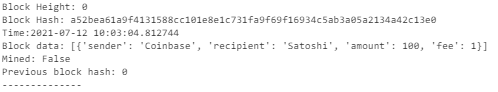
\includegraphics[width=0.9\textwidth]{../../Figures/genesis_block.png}
\end{center}
\end{frame}

\begin{frame}{Protocole de consensus}
Mécanisme pour permettre aux noeuds du réseau de s'accorder sur les informations à inclure dans les blocs.\\
\vspace{0.3cm}
Trois dimensions à analyser
\begin{enumerate}
  \item Efficacité 
  \item Décentralisation
  \item Sécurité 
  
\end{enumerate}
\footnotesize
\begin{thebibliography}{1}
\bibitem{Fu2020}
X.~Fu, H.~Wang, and P.~Shi, ``A survey of blockchain consensus algorithms:
  mechanism, design and applications,'' {\em Science China Information
  Sciences}, vol.~64, nov 2020.
\end{thebibliography}

\end{frame}
\begin{frame}{Preuve de travail}
Les noeuds sont en concurrence pour trouver la solution d'un problème via un procédé de type essai/erreur.
\begin{tcolorbox}[enhanced,drop shadow, title=PoW]
\begin{enumerate}
    \item Choisir une nombre aléatoire (nonce)
    \[
    X\sim\{1,\ldots, 2^{32}\}.
    \]
    \item Tant que $X > L$, où $L$ correspond à la difficulté on recommence  
\end{enumerate}
\end{tcolorbox}
\vspace{0.3cm}
Les noeuds sont choisis en fonction de leur puissance de calcul.
{\footnotesize
\begin{thebibliography}{1}
\bibitem{Na08}
S.~Nakamoto, ``Bitcoin: A peer-to-peer electronic cash system.'' Available at
  \href{https://bitcoin.org/bitcoin.pdf}{https://bitcoin.org/bitcoin.pdf},
  2008.
\end{thebibliography}  
}
\end{frame}
\begin{frame}{Usage de la blockchain: Les cryptomonnaies}
\begin{columns}
\begin{column}{0.5\textwidth}
   
{\footnotesize
\begin{thebibliography}{1}
\bibitem{Na08}
S.~Nakamoto, ``Bitcoin: A peer-to-peer electronic cash system.'' Available at
  \href{https://bitcoin.org/bitcoin.pdf}{https://bitcoin.org/bitcoin.pdf},
  2008.
\end{thebibliography}  
}
\end{column}
\begin{column}{0.5\textwidth}  %%<--- here
    \begin{center}
     
\includegraphics[width=0.5\textwidth]{../../Figures/bitcoin-6284869_1920.png}
     \end{center}
\end{column}
\end{columns}

\begin{itemize}
  \item Transactions anonymes
  \item Fournir une monnaie stable dans certaine région du monde
  \item Transferts de valeur internationaux 
  \item Pas d'autorité centrale
\end{itemize}
\end{frame}

\section{Théorie du risque en assurance}
\begin{frame}{Le modèle de ruine de Cramer-Lunberg}
\begin{columns}
\begin{column}{0.5\textwidth}
\scriptsize
La réserve financière d'une compagnie d'assurance est donnée par
\begin{equation*}
R_t = u +ct - \sum_{i = 1}^{N_t}U_i\text{, }t\geq0,
\end{equation*}
où 
\begin{itemize}
  \item $u>0$ est la réserve initial
  \item $c$ est le taux de prime
  \item $(N_t)_{t\geq0}$ est un processus de comptage égale au nombre de sinistres reportés à l'instant $t\geq0$
  \begin{itemize}
    \scriptsize
    \item[$\hookrightarrow$]  Processus de Poisson d'intensité $\lambda$
  \end{itemize}
  \item Les $U_i$ sont les indemnisations
  \begin{itemize}
    \scriptsize
    \item[$\hookrightarrow$] Suite de variables aléatoires positives, \textbf{i.i.d.}, et indépendantes de $N_t$
  \end{itemize}
\end{itemize}
\end{column}
\begin{column}{0.5\textwidth}
\begin{tikzpicture}
  %Origin and axis
  \coordinate (O) at (0,0);
  \draw[->] (-0.5,0) -- (5.5,0) coordinate[label = {below:\scriptsize$t$}] (xmax);
  \draw[->] (0,-0.5) -- (0,4) coordinate[label = {right:\scriptsize$R_t$}] (ymax);
   %Initial reserves
  \draw (0,2) node[black,left] {\scriptsize$u$} node{};
 % % %Length of the honest chain
  \draw[thick, tublue,-] (0,2) -- (2,3) node[pos=0.5, above] {};
  \draw[thick, dashed, tublue] (2,3) -- (2,1) node[pos=0.5, left] {\scriptsize\color{black}$U_1$};
  \draw[thick, tublue] (2,1) -- (3,1.5) node[pos=0.5, above] {};
  \draw[thick, dashed, tublue] (3,1.5) -- (3, 0.5) node[pos=0.5, left] {\scriptsize\color{black}$U_2$};
  \draw[thick, tublue] (3,0.5) -- (5, 1.5) node[pos=0.5, above] {};
   \draw[thick, dashed, tublue] (5,1.5) -- (5, -0.5) node[pos=0.5,above left] {\scriptsize\color{black}$U_3$};

  %Block finding Times 
  \draw (2,0) node[black,below] {\scriptsize$T_1$} node{ \color{black}$\bullet$};
  \draw (3,0) node[black,below] {\scriptsize$T_2$} node{ \color{black}$\bullet$};
  \draw (5,0) node[black,below left] {\scriptsize$\tau_z$} node{ \color{black}$\bullet$};
\end{tikzpicture}
\end{column}
\end{columns}

\end{frame}
\begin{frame}{Probabilités de ruine}
\scriptsize
Le temps de ruine est donné par
$$
\tau_u = \inf\{t\geq0\text{ ; }R_t <0\}
$$
et la probabilité de ruine par
$$
\psi(u,t) = \mathbb{P}(\tau_u < t)\text{ et }\psi(u) = \mathbb{P}(\tau_u < \infty)
$$
Trouver $u$ tel que 
$$
\mathbb{P}(\text{Ruin}) = \alpha\text{ (0.005)},
$$
avec
$$
c=(1+\eta)\lambda\mathbb{E}(U),
$$
où 
$$\eta>0\text{ (Condition de profitabilité)}$$  
sinon 
$$\psi(u)=1.$$

\tiny
\begin{thebibliography}{1}

\bibitem{Asmussen_2010}
S.~Asmussen and H.~Albrecher, {\em Ruin Probabilities}.
\newblock {WORLD} {SCIENTIFIC}, sep 2010.

\end{thebibliography}

\end{frame}


\section{Lien avec la blockchain}
\begin{frame}{Modèle de risque dual}
\begin{columns}
\begin{column}{0.5\textwidth}
\scriptsize
Soit un mineur 
\begin{itemize}
  \item dont la part de puissance de calcul est $p\in(0,1)$
  \item qui détient $u\geq0$ initialement 
  \item dépense $c = \pi_W\cdot W\cdot p$ par unité de temps
  \item trouve en moyenne $p \lambda$ blocs par unité de temps, où $\lambda$ est le nombre de bloc trouvés par l'ensemble du réseau
\end{itemize}
La richesse du mineur est donnée par
$$
R_t = u - c\cdot t + N_t\cdot b,\text{ (modèle de risque dual)}
$$
où 
\begin{itemize}
  \item $(N_t)_{t\geq0}$ est un processus de Poisson d'intensité $p\cdot\lambda$
  \item $b$ est la récompense associée à l'ajout d'un bloc (6.25 BTC) \url{bitcoinhalf.com}
\end{itemize}
\end{column}
\begin{column}{0.5\textwidth}
\begin{tikzpicture}
  %Origin and axis
  \coordinate (O) at (0,0);
  \draw[->] (-0.5,0) -- (5.5,0) coordinate[label = {below:\scriptsize$t$}] (xmax);
  \draw[->] (0,-0.5) -- (0,4) coordinate[label = {right:\scriptsize$R_t$}] (ymax);
   %Initial reserves
  \draw (0,3) node[black,left] {\scriptsize$u$} node{};
 % % %Length of the honest chain
  \draw[thick, tublue,-] (0,3) -- (2,1) node[pos=0.5, above] {};
  \draw[thick, dashed, tublue] (2,1) -- (2,2) node[pos=0.5, above left] {\scriptsize\color{black}$b$};
  \draw[thick, tublue] (2,2) -- (3.5,0.5) node[pos=0.5, above] {};
  \draw[thick, dashed, tublue] (3.5,0.5) -- (3.5, 1.5) node[pos=0.5, above left] {\scriptsize\color{black}$b$};
  \draw[thick, tublue] (3.5,1.5) -- (5, 0) node[pos=0.5, above] {};

  %Block finding Times 
  \draw (2,0) node[black,below] {\scriptsize$T_1$} node{ \color{black}$\bullet$};
  \draw (3.5,0) node[black,below] {\scriptsize$T_2$} node{ \color{black}$\bullet$};
  \draw (5,0) node[black,below] {\scriptsize$\tau_u$} node{ \color{black}$\bullet$};
\end{tikzpicture}
\end{column}
\end{columns}
\end{frame}
\begin{frame}{Profit espéré si solvabilité}
\scriptsize

\begin{tcolorbox}[enhanced,drop shadow, title=Remarque]
Le coût opérationel constant compensé par des récompenses peu fréquente rend l'activité de minage risquée.
\end{tcolorbox}
Le temps de ruine est défini par
$$
\tau_u  = \inf\{t\geq0\text{ ; }R_t \leq0\}
$$
\begin{itemize}
  \item Mesure de risque
  $$
  \psi(u,t) = \mathbb{P}(\tau_u \leq t)
  $$
  \item Mesure de performance
  $$
  V(u,t) = \mathbb{E}(R_t\mathbb{I}_{\tau_u > t})
  $$
\end{itemize} 
\end{frame}
\begin{frame}{Le dilemne du mineur} 
\scriptsize
$\psi$ and $V$ permette de comparer le minage individuel
\begin{itemize}
  \item au minage au sein d'un pool
\tiny
  \begin{thebibliography}{1}

\bibitem{rosenfeld2011analysis}
M.~Rosenfeld, ``Analysis of bitcoin pooled mining reward systems,'' 2011.

\bibitem{albrecher2021blockchain}
H.~Albrecher, D.~Finger, and P.-O. Goffard, ``Blockchain mining in pools:
  Analyzing the trade-off between profitability and ruin,'' 2021.


\end{thebibliography}
  \item \scriptsize à la déviation par rapport au protocole (minage égoïste)

  \tiny
  \begin{thebibliography}{1}
  \bibitem{Eyal2014}
I.~Eyal and E.~G. Sirer, ``Majority is not enough: Bitcoin mining is
  vulnerable,'' in {\em Financial Cryptography and Data Security},
  pp.~436--454, Springer Berlin Heidelberg, 2014.

\bibitem{albrecher:hal-02649025}
H.~Albrecher and P.-O. Goffard, ``{On the profitability of selfish blockchain
  mining under consideration of ruin},'' {\em To appear in Operations
  Research}, May 2021.
\newblock \url{https://arxiv.org/abs/2010.12577}.
\end{thebibliography}
\end{itemize}
Des formules analytiques sont données pour 
$$
\widehat{\psi}(u,t)= \mathbb{E}[\psi(u,T)]\text{ and }\widehat{V}(u,t)= \mathbb{E}[V(u,T)],
$$
où $T\sim\text{Exp}(t)$.
\end{frame}

\begin{frame}{Minage solo}
\scriptsize
\begin{tcolorbox}[enhanced,drop shadow, title=Theorem (profit and ruin when mining solo)]
Pour $u\geq0$, on a 
\begin{equation*}
\widehat{\psi}(u,t) = e^{\rho^\ast u},
\end{equation*}
et 
\begin{equation*}
\widehat{V}(u,t) = u+(p\lambda b-c)t\left(1-e^{\rho^\ast u }\right),
\end{equation*}
où $\rho^\ast$ est la solution négative de l'équation
\begin{equation}\label{eq:equation_rho}
-c\rho + p\lambda(e^{b\rho}-1) = 1/t.
\end{equation}
\end{tcolorbox}
\begin{tcolorbox}[enhanced,drop shadow, title=Lambert function]
La solution $\rho^\ast$ de \eqref{eq:equation_rho} est donnée par 
\begin{equation*}
  \rho^{\ast}=-\frac{p \lambda t+1}{ct}
  -\frac{1}{b} \,{\rm W} \left[-\frac{p\lambda
    \,b}{c}\,{e^{-b\,\left(\frac{p \lambda t+1}{ct}\right)}}
  \right],
  \end{equation*}
  où $W(.)$ désigne la fonction de Lambert.
\end{tcolorbox}
\end{frame}
\begin{frame}{Elements de preuve}
\scriptsize
L'horizon de temps est aléatoire avec $T\sim\text{Exp}(t)$, on réalise un bilan de probabilité sur l'intervalle $(0,h)$, avec $h<u/c$ ce qui rend la ruine impossible avant $h$. Trois possibilités
\begin{itemize}
  \item[(i)] $T>h$ et pas de nouveau bloc sur $(0,h)$
  \item[(ii)] $T<h$ et pas de nouveau bloc sur $(0,T)$
  \item[(iii)] Un bloc est découvert avant $T$ et $h$
\end{itemize}
Pour la richesse espérée $\widehat{V}(u,t)$, on a 
\begin{eqnarray*}
  \widehat{V}(u,t)& =&e^{-h(1/t + p\lambda)}\,\widehat{V}(u-ch,t)+\int\limits_0^h\frac1t\, e^{-s(1/t + p\lambda)}\,(u-cs)ds\\
  &+&\int\limits_0^h p\lambda\, e^{-s(1/t + p\lambda)}\,\widehat{V}(u-cs+b,t)ds.
  \end{eqnarray*}
  \end{frame}
\begin{frame}{Elements de preuve}
\scriptsize
On dérive par rapport à $h$ et on prend $h=0$ pour obtenir
\begin{equation}\label{eq:ODE}
c\widehat{V}'(u,t) + \left(\frac{1}{t} +  p\lambda\right)\widehat{V}(u,t) - p\lambda \widehat{V}(u+b,t) - \frac{u}{t} =0,
\end{equation}
L'équation \eqref{eq:ODE} est une équation différentielle avec avance
\blfootnote{\tiny 
 H.~L. Smith, {\em An introduction to delay differential equations with
  applications to the life sciences}.
\newblock Springer, New York, 2011.
}
Les conditions limites sont
$$
\widehat{V}(0,t) = 0 \text{ et tel que } 0\leq \widehat{V}(u,t)\leq u-ct+p\lambda b t \text{ pour }u>0.
$$  
Considérons les solutions de la forme 
\begin{equation}\label{eq:potential_solution}
\widehat{V}(u,t) = Ae^{\rho u }+Bu + C,\text{ }u \ge 0, 
\end{equation}
où $A, B,C$ et $\rho$ sont des constantes à déterminer. La substitution de  \eqref{eq:potential_solution} dans \eqref{eq:ODE} en tenant compte des conditions initiales mène au système d'équations
\begin{equation*}
\begin{cases}
0&=ct\rho + \left(1+p\lambda t\right)-p\lambda te^{\rho b}, \\
0&= B\left(1+tp\lambda\right)-p\lambda tB - 1,\\
0&=Bct+C(1+tp\lambda) - p\lambda t Bb-p\lambda tC, \\
0&=A+C.
\end{cases}
\end{equation*}
\end{frame}
\begin{frame}{Elements de preuve}
\scriptsize
On obtient $A = -t(p\lambda b - c)$, $B = 1$, $C = t(p\lambda b - c)$ et $\rho$ solution de
$$
c\rho + \left(1+p\lambda t\right)-p\lambda te^{\rho b} = 0,
$$
qui admet une solution négative et une solution positive. Comme $A<0$, nous devons prendre la solution négative  $\rho^\ast<0$ pour satisfaire la condition $\widehat{V}(u,t)>0$. La substitution de $A,B,C$ et $\rho^{\ast}$ dans \eqref{eq:potential_solution} renvoie le résultat.\\

De manière analogue, la probabilité de ruine vérifie 
\begin{equation*}\label{psii}
c\widehat{\psi}'(u,t)+(p \lambda+1/t)\,\widehat{\psi}(u,t)-p \lambda\,\widehat{\psi}(u+b,t)=0
\end{equation*}
avec les conditions initiales $\widehat{\psi}(0,t)=1$ et la condition limite $\lim_{u\to\infty}\widehat{\psi}(u,t)=0$.
\end{frame}
\begin{frame}{Comment fonctionne un pool de minage ?}
\scriptsize
Un ensemble de mineurs $I\subset\{1,\ldots, n\}$ totalise une proportion 
$$
p_I = \sum_{i\in I }p_i,
$$
de la puissance de calcul du réseau. 
\begin{itemize}
  \item Un gestionnaire coordonne cette association
  \item Les mineurs prouvent leur contributions en soumettant des solutions partielles (\textit{parts})  
\end{itemize}
Le gestionnaire décide
\begin{itemize} 
  \item du système de rémunération
  \item de la difficulté relative $q\in(0,1)$ de trouver une \textit{part} plutôt qu'une vraie solution
  \item des frais de participation $f$
  \end{itemize} 
\end{frame}
\begin{frame}{Système de redistribution}
\scriptsize
Les mineurs doivent être rémunéré à hauteur de leur contribution à l'effort de minage. 
\begin{tcolorbox}[enhanced,drop shadow, title=Rémunération proportionnel]
Un \text{tour} est le temps séparant la découvert de deux blocs 
\begin{itemize} 
  \item $s_i$ est le nombre de \textit{parts} soumis par le mineur $i\in I$ durant le \textit{tour}
  \item Chaque mineur reçoit à la fin du \textit{tour}
  $$
  (1-f)\cdot b\cdot\frac{s_i}{\sum_{i\in I}s_i},
  $$
  où $f$ représente le taux de frais perçu par le gestionnaire.
  \item Le système est dit juste si $\frac{s_i}{\sum_{i\in I}s_i}$ converge vers $\frac{p_i}{\sum_{i\in I}p_i}$
\end{itemize}

\end{tcolorbox}
\end{frame}
\begin{frame}{Le problème du sytème proportionnel}
\scriptsize
\begin{tcolorbox}[enhanced,drop shadow, title=Remarque]
Le système de rémunération proportionnel est juste mais pas incitatif.
\end{tcolorbox}
\tiny
\begin{thebibliography}{1}

\bibitem{Schrijvers2017}
O.~Schrijvers, J.~Bonneau, D.~Boneh, and T.~Roughgarden, ``Incentive
  compatibility of bitcoin mining pool reward functions,'' in {\em Financial
  Cryptography and Data Security}, pp.~477--498, Springer Berlin Heidelberg,
  2017.

\end{thebibliography}
\scriptsize

\begin{itemize}
  \item La durée des \textit{tours} est aléatoire 
  \begin{itemize}
    \scriptsize
    \item[$\hookrightarrow$] Une \textit{part} perd de la valeur lorsque le \textit{tour} s'éternise $\Rightarrow$ \textit{pool hoping} \tiny
    \begin{thebibliography}{1}

\bibitem{rosenfeld2011analysis}
M.~Rosenfeld, ``Analysis of bitcoin pooled mining reward systems,'' 2011.

\end{thebibliography}
\scriptsize
    \item[$\hookrightarrow$] Appliquer un facteur d'actualisation à la valeur des \textit{parts} \tiny
    \begin{thebibliography}{1}
\bibitem{slush}
slush pool, ``Reward system specifications,'' 2021.
\end{thebibliography}
  \end{itemize}
  \item Un mineur peut retarder la communication d'une solution
  \begin{itemize}
    \scriptsize
    \item[$\hookrightarrow$] Pour attendre que son taux de \textit{part} soit en accord avec sa puissance de calcul 
  \end{itemize} 
  \item Aucun transfert de risque des mineurs vers le gestionnaire
    \begin{itemize}
    \scriptsize
    \item[$\hookrightarrow$] $f$ doit être minimale
  \end{itemize} 
\end{itemize}
\end{frame}
\begin{frame}{Le système Pay-per-Share (PPS) }
\scriptsize
Le gestionnaire paie
$$
w = (1-f)\cdot q \cdot b 
$$ 
pour chaque \textit{part} et conserve l'intégralité de la récompense des blocs.
\vspace{1cm}
\begin{columns}
\begin{column}{0.5\textwidth}
Richesse du mineur
$$
R_t^i = u_i-ct + M_t^i w,\text{ }t\geq0.
$$
où 
\begin{itemize}
   \item $(M_t^i)_{t\geq0}$ est un processus de Poisson d'intensité $p_i \mu= p_i\lambda / q$
   \item $\mu$ correspond au nombre moyen de \textit{parts} soumises par le réseau 
\end{itemize}
\end{column}
\begin{column}{0.5\textwidth}
Richesse du gestionnaire
$$
R_t^I = u_I - M_t^I w+N_t^I b,\text{ }t\geq0.
$$
où 
\begin{itemize}
   \item $(M_t^I)_{t\geq0}$ est un processus de Poisson d'intensité $p_I\mu =p_I\lambda / q$
   \item $(N_t^I)_{t\geq0}$ est un processus de Poisson d'intensité $p_I\lambda$
\end{itemize}
\end{column}
\end{columns}
\end{frame}
\begin{frame}{Risque du gestionnaire}
\scriptsize
On remplace les récompenses déterministes par des récompenses aléatoires, la richesse du gestionnaire devient
$$
R_t= u - \sum_{i=1}^{M_t} W_i +\sum_{j=1}^{N_t} B_j,\text{ }t\geq0.
$$
où 
\begin{itemize}
  \item $(M_t)_{t\geq0}$ et $(N_t)_{t\geq0}$ sont des processus de Poisson d'intensité respective $\mu^\ast=\mu- \lambda$ et $\lambda$
  \item $(W_i)_{i\geq0}$ et $(B_j)_{j\geq0}$ sont deux suites indépendantes de variables aléatoires  \iid  de loi exponentielle ode moyenne $w$ et $b^\ast = b-w$.
\end{itemize}
\begin{tcolorbox}[enhanced,drop shadow, title=Superposition de processus de Poisson]
La découverte d'un bloc est associé au paiement d'une part aux mineurs
\begin{itemize}
\item L'intensité de $M_t$ est donnée par $\mu^\ast=\mu- \lambda$ 
\item La moyenne des récompense pour la découverte d'un bloc est donnée par $b^\ast = b-w$ 
\end{itemize}
Cela permet de distinguer les sauts vers le haut et vers le bas tout en rendant les processus de Poisson indépendants. 
\end{tcolorbox}
\end{frame}
\begin{frame}{Risque du gestionnaire}
\scriptsize
\begin{tcolorbox}[enhanced,drop shadow, title=Théorème (Pertes et profits du gestionnaire)]
La probabilité de ruine est donnée par 
\begin{equation*}\label{psiexpe}
    \widehat{\psi}(u,t) = (1-Rw)  e^{-R u},\;u\ge 0,
\end{equation*}
et la richesse espéré par
\begin{equation*}\label{Vcombexpe}
    \w{V}(u,t) = (1 - Rw)[w-t(\lambda b^\ast-\mu^\ast w)] e^{-R u}+u+t(\lambda b^\ast-\mu^\ast w),
\end{equation*}
où $R$ est la seule solution 
\begin{equation*} \label{VLunde}
    -(t^{-1}+\lambda+\mu^\ast)+\lambda(1+b^\ast r)^{-1}+\mu^\ast(1-wr)^{-1}=0.
\end{equation*}
de partie réelle positive.
\end{tcolorbox}
\tiny
  \begin{thebibliography}{1}

\bibitem{albrecher2021blockchain}
H.~Albrecher, D.~Finger, and P.-O. Goffard, ``Blockchain mining in pools:
  Analyzing the trade-off between profitability and ruin,'' 2021.


\end{thebibliography}
\end{frame}
\begin{frame}[allowframebreaks]{Elements de preuve}
\scriptsize
Bilan de probabilité sur l'intervalle $(0,h)$. Quatre possibilités
\begin{itemize}
  \item[(i)] $T>h$ et pas de saut sur $(0,h)$
  \item[(ii)] $T<h$ et pas de saut sur $(0,T)$
  \item[(iii)] Un saut vers le haut sur $(0,h)$
  \item[(iv)] Un saut vers le bas sur $(0,h)$
\end{itemize}
  \begin{eqnarray*}\label{neu0}
      \w{V}(u,t)&=& e^{-(\frac{1}{t}+\lambda+\mu^\ast)h}\w{V}(u,t) + \frac{1}{t}\int_0^h e^{-{s}/{t}}e^{-(\lambda +\mu^\ast) s} u\,ds\\
      & +& \lambda\int_0^he^{-\lambda s} e^{-({1}/{t}+\mu^\ast) s} \int_0^\infty\w{V}(u+x,t)\,dF_{B}(x)\,ds\\
      &  +&\mu^\ast \int_0^he^{-\mu^\ast s} e^{-({1}/{t}+\lambda) s}\int_0^u \w{V}(u-y,t) \,dF_W(y)\,ds.
  \end{eqnarray*}
  On dérive par rapport à $h$ et on fait tendre $h\rightarrow 0$, ce qui mène à l'équation intégrale
  \begin{equation} \label{inteq}
    \lambda\int_0^\infty\w{V}(u+x,t)\,dF_{B}(x)-(\lambda+\mu^\ast+{1}/{t})\w{V}(u,t)+\mu^\ast\int_0^u \w{V}(u-y,t) \,dF_W(y)+{u}/{t}=0,\quad u\ge 0,
  \end{equation}
  munie des conditions initiales $\w{V}(u,t)=0$ pour tout $u<0$ et $0\leq\w{V}(u,t)\leq u+(\lambda b^\ast - \mu^\ast w)t$. On considère des solutions de la forme
  $$
  Ce^{-ru}+d_1u+d_0
  $$
  \begin{itemize}
    \item Par comparaison des termes en $e^{-r u}$ on obtient une équation pour $r$ avec
    $$
    -(t^{-1}+\lambda+\mu^\ast)+\lambda(1+b^\ast r)^{-1}+\mu^\ast(1-wr)^{-1}=0
    $$
    dont l'unique solution positive $R>0$ est valide au vu de la borne $0\leq\w{V}(u,t)\leq u+(\lambda b^\ast - \mu^\ast w)t$
    \item Par comparaison des termes en $u$, il vient $d_1 = 1$
    \item Par comparaison des termes en $1$ il vient
    $$
    d_0 = t(\lambda b^\ast-\mu^\ast w)
    $$
    \item Par comparaison des termes en $e^{-u/w}$, on a
    $$
    C = (1 - Rw)[w-t(\lambda b^\ast-\mu^\ast w)]
    $$
  \end{itemize}
\end{frame}
\begin{frame}{Problèmes liés au minage}
\begin{itemize}
  \item Course à l'armement, Consomation électrique importante et génération de e-déchet
\tiny
\begin{thebibliography}{1}

\bibitem{bertucci2020mean}
C.~Bertucci, L.~Bertucci, J.-M. Lasry, and P.-L. Lions, ``Mean field game
  approach to bitcoin mining,'' 2020.

\bibitem{Alsabah2018}
H.~Alsabah and A.~Capponi, ``Bitcoin mining arms race: R{\&}d with
  spillovers,'' {\em {SSRN} Electronic Journal}, 2018.

\end{thebibliography}
\end{itemize}
\begin{itemize}
  \item \normalsize Une menace sur la décentralisation?
\tiny
\begin{thebibliography}{1}

\bibitem{Cong2020}
L.~W. Cong, Z.~He, and J.~Li, ``Decentralized mining in centralized pools,''
  {\em The Review of Financial Studies}, vol.~34, pp.~1191--1235, apr 2020.

\bibitem{li2019mean}
Z.~Li, A.~M. Reppen, and R.~Sircar, ``A mean field games model for
  cryptocurrency mining,'' 2019.

\end{thebibliography}
\end{itemize}
\end{frame}


\end{document}
